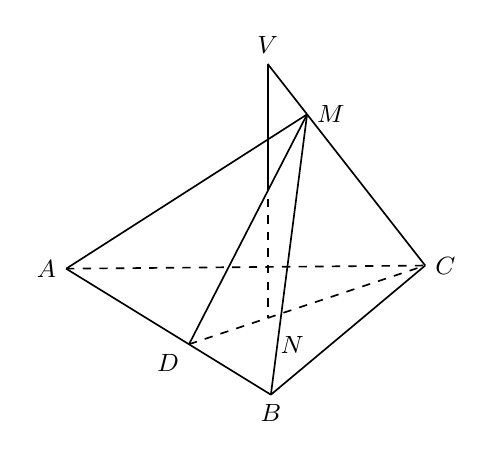
\begin{tikzpicture}[line width=0.6pt, font=\small]
  \coordinate (A) at (0,1.6);
  \coordinate (B) at (2.6,0);
  \coordinate (C) at (4.56,1.64);
  \coordinate (D) at (1.5600000000,0.6400000000);
  \coordinate (N) at (2.5600000000,0.9733333333);
  \coordinate (V) at (2.5600000000,4.2000000000);
  \coordinate (M) at (3.0600000000,3.5600000000);
  % base: AB via D solid, BC solid, AC dashed
  \draw (A) -- (D) -- (B);
  \draw (B) -- (C);
  \draw[dashed] (A) -- (C);
  % altitude CD dashed (D-N-C collinear)
  \draw[dashed] (D) -- (C);
  % vertical VN dashed
  \draw (V)--(2.5599999999999996,2.7);\draw[dashed] (2.5599999999999996,2.7)--(N);
  % skew edge VC via M solid
  \draw (V) -- (M) -- (C);
  % segments from M solid
  \draw (A) -- (M);
  \draw (D) -- (M);
  \draw (B) -- (M);
  % labels
  \node[left] at (A) {$A$};
  \node[below] at (B) {$B$};
  \node[right] at (C) {$C$};
  \node[below left] at (D) {$D$};
  \node[below right,xshift=1pt,yshift=-3pt] at (N) {$N$};
  \node[above] at (V) {$V$};
  \node[right] at (M) {$M$};
\end{tikzpicture}
